\documentclass{beamer}
\mode<presentation>
\usepackage{amsmath}
\usepackage{amssymb}
%\usepackage{advdate}
\usepackage{graphicx}
\graphicspath{{./figs/}}
\usepackage{adjustbox}
\usepackage{subcaption}
\usepackage{enumitem}
\usepackage{multicol}
\usepackage{mathtools}
\usepackage{listings}
\usepackage{url}
\def\UrlBreaks{\do\/\do-}
\usetheme{Boadilla}
\usecolortheme{lily}
\setbeamertemplate{footline}
{
  \leavevmode%
  \hbox{%
  \begin{beamercolorbox}[wd=\paperwidth,ht=2.25ex,dp=1ex,right]{author in head/foot}%
    \insertframenumber{} / \inserttotalframenumber\hspace*{2ex} 
  \end{beamercolorbox}}%
  \vskip0pt%
}
\setbeamertemplate{navigation symbols}{}

\providecommand{\nCr}[2]{\,^{#1}C_{#2}} % nCr
\providecommand{\nPr}[2]{\,^{#1}P_{#2}} % nPr
\providecommand{\mbf}{\mathbf}
\providecommand{\pr}[1]{\ensuremath{\Pr\left(#1\right)}}
\providecommand{\qfunc}[1]{\ensuremath{Q\left(#1\right)}}
\providecommand{\sbrak}[1]{\ensuremath{{}\left[#1\right]}}
\providecommand{\lsbrak}[1]{\ensuremath{{}\left[#1\right.}}
\providecommand{\rsbrak}[1]{\ensuremath{{}\left.#1\right]}}
\providecommand{\brak}[1]{\ensuremath{\left(#1\right)}}
\providecommand{\lbrak}[1]{\ensuremath{\left(#1\right.}}
\providecommand{\rbrak}[1]{\ensuremath{\left.#1\right)}}
\providecommand{\cbrak}[1]{\ensuremath{\left\{#1\right\}}}
\providecommand{\lcbrak}[1]{\ensuremath{\left\{#1\right.}}
\providecommand{\rcbrak}[1]{\ensuremath{\left.#1\right\}}}
\theoremstyle{remark}
\newtheorem{rem}{Remark}
\newcommand{\sgn}{\mathop{\mathrm{sgn}}}
\providecommand{\abs}[1]{\left\vert#1\right\vert}
\providecommand{\res}[1]{\Res\displaylimits_{#1}} 
\providecommand{\norm}[1]{\lVert#1\rVert}
\providecommand{\mtx}[1]{\mathbf{#1}}
\providecommand{\mean}[1]{E\left[ #1 \right]}
\providecommand{\fourier}{\overset{\mathcal{F}}{ \rightleftharpoons}}
%\providecommand{\hilbert}{\overset{\mathcal{H}}{ \rightleftharpoons}}
\providecommand{\system}[1]{\overset{\mathcal{#1}}{ \longleftrightarrow}}
%\providecommand{\system}{\overset{\mathcal{H}}{ \longleftrightarrow}}
	%\newcommand{\solution}[2]{\textbf{Solution:}{#1}}
%\newcommand{\solution}{\noindent \textbf{Solution: }}
\providecommand{\dec}[2]{\ensuremath{\overset{#1}{\underset{#2}{\gtrless}}}}
\newcommand{\myvec}[1]{\ensuremath{\begin{pmatrix}#1\end{pmatrix}}}
\let\vec\mathbf

\lstset{
%language=C,
frame=single, 
breaklines=true,
columns=fullflexible
}

\numberwithin{equation}{section}
\title{2.6.38}
\author{AI25BTECH11027 - NAGA BHUVANA}
% \maketitle
% \newpage
% \bigskip
\begin{document}
{\let\newpage\relax\maketitle}
\renewcommand{\thefigure}{\theenumi}
\renewcommand{\thetable}{\theenumi}
\noindent
		\textbf{Question:}\\
If $\vec{a}=\hat{i}+\hat{j}+\hat{k}$ and $\vec{b}=\hat{j}-\hat{k}$, find a vector $\vec{c}$ such that $\vec{a} \times \vec{c}=\vec{b}$ and $\vec{a} \cdot \vec{c}=3$\\
\textbf{Solution:}\\
\begin{align}
\vec{a}=\myvec{1\\1\\1},\vec{b}=\myvec{0\\1\\-1}
\end{align}
    \begin{align}
        \vec{a}^T\vec{c}=3\\
        \vec{b}^T\vec{c}=0
    \end{align}
    \begin{align}
        \myvec{\vec{a} && \vec{b}}^T\vec{c}=\myvec{3\\0}
    \end{align}
   \begin{align}
       \myvec{1&1&1\\0&1&-1}\vec{c}=\myvec{3\\0}
   \end{align}
   By solving\\
   \begin{align}
       \vec{c}=\myvec{3\\0\\0}+\lambda \myvec{-2\\1\\1}=\myvec{3-2\lambda \\ \lambda \\ \lambda}
   \end{align}
   \begin{align}
	   \lambda=\frac{2}{3} \quad \text{Satisfies the cross product condition}
   \end{align}
\begin{align}
    \vec{c}=\myvec{\frac{5}{3}\\ \frac{2}{3}\\ \frac{2}{3}}
\end{align}
\begin{align}
    \therefore \vec{c}=\frac{5}{3}\hat{i}+\frac{2}{3}\hat{j}+\frac{2}{3}\hat{k}
\end{align}
\begin{frame}
	\frametitle{Graphical Representation}
	\centering
	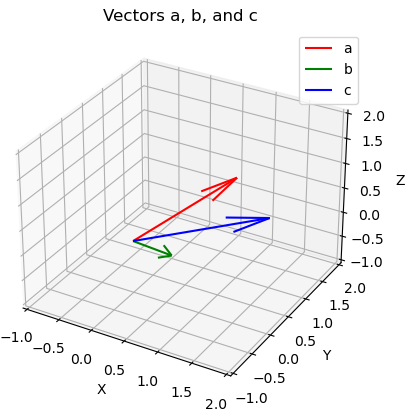
\includegraphics[width=0.7\linewidth]{figs/fig1.png}
\end{frame}
\end{document}
